\begin{frame}
\frametitle{Truck platoon models near a merge}
\metroset{block=fill}
    \smartdiagramset{description title width=1.2cm, 
            description title text width=2cm}
    \onslide<1->{        
    \begin{columns}
      \begin{column}{0.6\linewidth}
        \smartdiagram[descriptive diagram]{
          {\textit{\textbf{Assumption}},{\structure{V2V/V2I} full connectivity}},
          {\textit{\textbf{Objective}}, {\structure{Safety} at the merge condition, + \alert{smoothed traffic} in main lane/ carrigeway}},
        }
      \end{column}
      \begin{column}{0.2\linewidth}
        \begin{figure}
          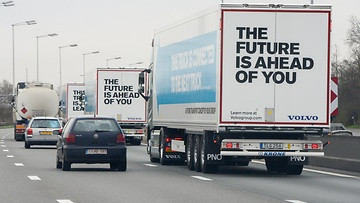
\includegraphics[width=\linewidth]
          {fig_25_truck-platoon-cutin}
        \end{figure}
      \end{column}
    \end{columns}
    }
    \onslide<2->{
    \begin{block}{Anticipated maneuver}
      \begin{description}
        \item[Detection] Measurement / detection of vehicles far upstream 
        \item[Yielding] Coordinated deccelearation between all trucks. 
        \item[Insertion] Smooth insertion   
      \end{description}
    \end{block}
    }
\end{frame}
